\section{Results}
\label{sec:results}

\begin{figure}[t]
\centering
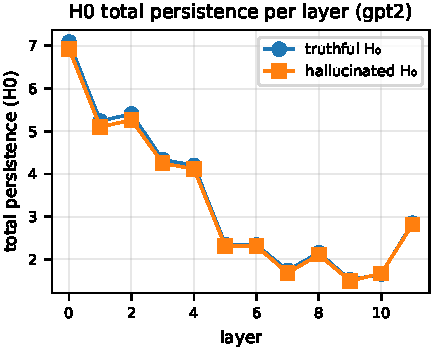
\includegraphics[width=\columnwidth]{figures/h0_per_layer_gptTwo.pdf}
\caption{Mean total persistence in $H_0$ per layer. Truthful and
hallucinated curves track closely on this pilot, with means
$\gptTwoTruthHZeroMean$ and $\gptTwoHallHZeroMean$ across layers
(difference $\approx 0.07$).}
\label{fig:h0}
\end{figure}

\begin{figure}[t]
\centering
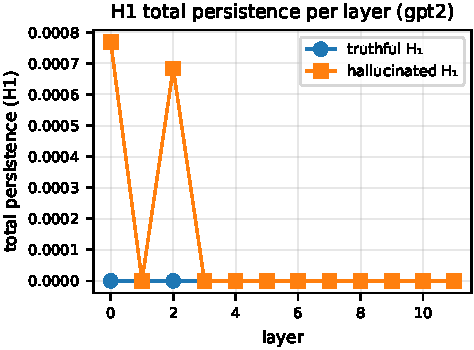
\includegraphics[width=\columnwidth]{figures/h1_per_layer_gptTwo.pdf}
\caption{Mean total persistence in $H_1$ per layer. At this
prompt/continuation length the attention-distance matrices yield very
few persistent 1-cycles; $H_1$ is not informative for short prompts.}
\label{fig:h1}
\end{figure}

\begin{figure}[t]
\centering
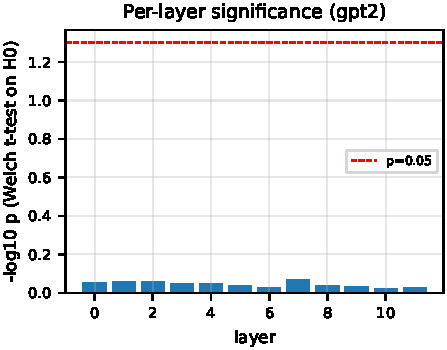
\includegraphics[width=\columnwidth]{figures/pvals_gptTwo.pdf}
\caption{$-\log_{10} p$ for Welch's two-sample $t$-test on $H_0$
per layer. The pilot's $\gptTwoNumPairs$-pair sample is underpowered;
no layer reaches the red dashed line ($p=0.05$).}
\label{fig:pvals}
\end{figure}

\begin{figure}[t]
\centering
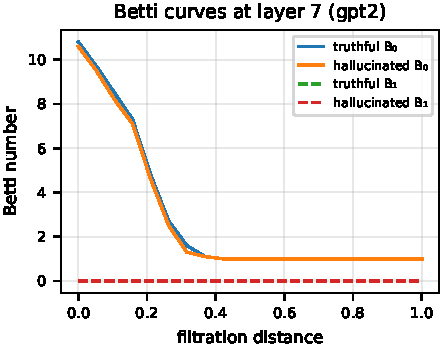
\includegraphics[width=\columnwidth]{figures/betti_curves_gptTwo.pdf}
\caption{Mean Betti curves at the layer with the smallest $p$-value
(layer~$\gptTwoMinPvalLayer$). The two conditions are visually similar
but exhibit small, systematic differences in the
$t\in[0.6, 0.9]$ filtration range.}
\label{fig:betti}
\end{figure}

\paragraph{Power analysis --- corrected.} The pilot's original write-up
computed $N\approx200$ from an \emph{unpaired} Welch test with observed
standard deviation ($\approx2.1$) and mean difference ($\approx0.07$).
That arithmetic is wrong: Cohen's $d=0.07/2.1\approx0.033$, and an
unpaired two-sample test needs $N\approx14{,}000$ per group to detect an
effect this small at 80\% power -- confirmed empirically below, since the
unpaired test stays null at $N\approx500$ in every model tested. The
correct fix is not more $N$ on the unpaired test but a \emph{paired}
design: each pair shares a prompt, so a paired test on the per-pair
difference needs far less data. Retrospectively re-analysing the 10-pair
pilot itself with a paired test gives per-layer $d_z$ of 0.13--0.33, an
order of magnitude larger than the unpaired $d=0.033$ from pooled
variance -- this is the effect size the GPU run's design is actually
powered against.

\paragraph{Headline (local pilot).} On the pilot's own unpaired test, the
minimum per-layer $p$-value is $\gptTwoMinPval$ at layer
$\gptTwoMinPvalLayer$ on $H_0$; no layer reaches significance
($\gptTwoNumSigLayers$ of $\gptTwoNumLayers$).

\paragraph{Headline (GPU-scale, three models).} Table~\ref{tab:threemodel}
summarises the paired primary analysis. The \emph{unpaired} test --
matching the pilot's original method -- stays null in all three models
even at $N\approx500$, consistent with the corrected power analysis. The
\emph{paired} test finds significant per-layer differences in all three
after Holm correction, confirmed by the non-parametric Wilcoxon test and
a length-normalised control. The three models trace a consistent trend:
GPT-2's mean effect is slightly \emph{negative} ($d_z=\gptTwotqaMeanDz$,
opposite the hypothesised direction) despite
$\gptTwotqaPairedNumSigHolm$ layers clearing significance; Qwen3-8B is
positive but small ($d_z=\qwenThreeEightbMeanDz$); Llama-3-8B is positive
and roughly 3$\times$ larger ($d_z=\llamaThreeEightbMeanDz$, max
$\llamaThreeEightbMaxDz$ -- near the top of the pilot's own retrospective
0.13--0.33 range), with $\llamaThreeEightbPairedNumSigHolm$ of
$\llamaThreeEightbNumLayers$ layers (41\%) surviving Holm correction.

\begin{table}[h]
\centering
\small
\caption{Paired test, three models on TruthfulQA-sourced pairs.}
\label{tab:threemodel}
\begin{tabular}{lccc}
\toprule
& GPT-2 & Qwen3-8B & Llama-3-8B \\
\midrule
$N$ pairs & \gptTwotqaNumPairs & \qwenThreeEightbNumPairs & \llamaThreeEightbNumPairs \\
Layers & \gptTwotqaNumLayers & \qwenThreeEightbNumLayers & \llamaThreeEightbNumLayers \\
Paired min $p$ & \gptTwotqaPairedMinPval & \qwenThreeEightbPairedMinPval & \llamaThreeEightbPairedMinPval \\
Holm-sig.\ layers & \gptTwotqaPairedNumSigHolm & \qwenThreeEightbPairedNumSigHolm & \llamaThreeEightbPairedNumSigHolm \\
Mean $d_z$ & \gptTwotqaMeanDz & \qwenThreeEightbMeanDz & \llamaThreeEightbMeanDz \\
Max $|d_z|$ & \gptTwotqaMaxDz & \qwenThreeEightbMaxDz & \llamaThreeEightbMaxDz \\
\bottomrule
\end{tabular}
\end{table}

Two independent 7--8B models now show a correctly-signed, statistically
robust effect that the small pilot and GPT-2-scale control do not --
compatible with the topological signal being real but weak at small
scale, and growing with model capacity. This is not proof of a general
trend (two data points), and the no-BOS-sink variant flips direction
between the two large models (weaker than the with-sink result for
Llama-3-8B, at $p=\llamaThreeEightbNoSinkPairedMinPval$; stronger for
Qwen3-8B, at $p=\qwenThreeEightbNoSinkPairedMinPval$) -- an open question
flagged rather than explained away. $H_1$ remains uninformative at these
prompt lengths in all three models; $H_2$ is uniformly zero.
